Quelle:\\ \href{http://drops.dagstuhl.de/opus/volltexte/2015/4944/pdf/44.pdf}{Visibly Counter Languages and Constant Depth Circuits, Krebs, Lange, Ludwig}
\section{Rückblick}
    Was wir von reg. Sprachen wissen:
    \begin{itemize}
        \item $\Reg$ ist $NC^1$-vollst.
        \item $\Reg\cap AC^0 = FO[Reg.]$
        	= quasi aper. $\gamma:\Sigma^*\to Synt(L)$
        \item $L\in \Reg\setminus AC^0 \Rightarrow L \text{ ist } ACC^0 \text{-schwer}$ (Dichotomie)
        \item $AC^0 \subsetneq ACC_k^0 \subseteq TC^0 \subseteq NC^1 \subseteq L \subseteq NL$\\[1mm]
            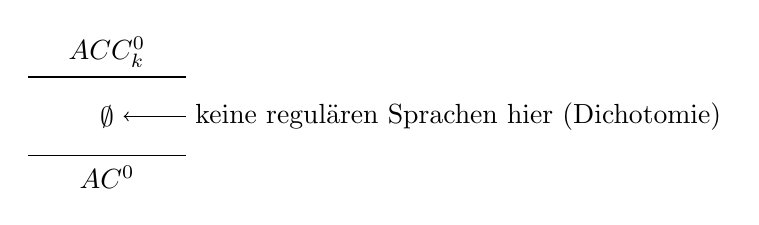
\begin{tikzpicture}
                \draw (0,1) -- (2,1) node[midway, above] (acc) {$ACC_k^0$};
                \node at (1,0.5) (empty) {$\emptyset$};
                \draw [<-] (empty) -- (2,0.5) node [anchor= west] {keine regulären Sprachen hier (Dichotomie)};
                \draw (0,0) -- (2,0) node[midway, below] (ac0) {$AC^0$};
            \end{tikzpicture}
        \item VPL auch $NC^1$-vollständig, also auch $VCL$.
    \end{itemize}
\section{Definition}
    $k-VCA:\ \mathcal{A} = (Q, q_0, E, \Sigma, \delta_0, \dots, \delta_k)$ mit $\delta_i = Q \times \Sigma \to \Sigma$ \\($i$ je nach Ebene, ab Ebene $m$ $\delta_k$)\\[2mm]
    Akzeptanzkriterium: Endzustand in Lauf erreichbar\\
    $\delta_{min}(m, \Delta(w))$ wird angewandt, nachdem $w$ gelesen wurde. $\Delta(w) = |w|_{call} - |w|_{return}$\\
    \begin{tikzpicture}
        \draw[->] (0,0) -- (0,3);
        \node at (0,1) [anchor=east] (m) {$\delta_m$};
        \draw[dotted] (m) -- (4,1);
        \draw[gray!50] (0,0) -- (1,2) -- (2,1) -- (3,3) -- (4,0);
        \fill[gray!20, pattern=north east lines] (0.5,1) -- (1,2) -- (2,1) -- (3,3) -- (3.667,1) -- cycle;
        \draw[->] (0,0) -- (4,0);
    \end{tikzpicture}
    \subsection{Beispiel}
        \begin{itemize}
            \item $a^nb^n \in 1-VCL$\\
                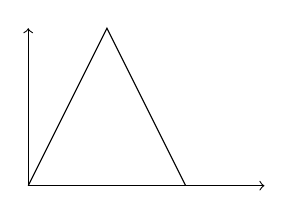
\begin{tikzpicture}
                    \draw[->] (0,0) -- (0,2);
                    \draw[->] (0,0) -- (3,0);
                    \draw (0,0) -- (1,2) -- (2,0);

                    % \draw[->] (4,0) -- (4,2);
                    % \draw[->] (4,0) -- (8,0);
                    % \draw (4,0) -- (4.5,2) -- (5,1) -- (5.5,2) -- (6,1) -- (6.5,2) -- (7,0);
                \end{tikzpicture}
            \item $a^nb^{n-3}a^mb^{m+3} \in 4-VCL$\\
                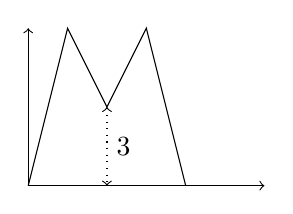
\begin{tikzpicture}
                    \draw[->] (0,0) -- (0,2);
                    \draw[->] (0,0) -- (3,0);
                    \draw (0,0) -- (0.5,2) -- (1,1) -- (1.5,2) -- (2,0);
                    \draw[<->,dotted] (1,1) -- (1,0) node[midway, right] {$3$};
                \end{tikzpicture}
        \end{itemize}
    \subsection{Anmerkung}
        Nicht in $AC^0$:
            \begin{itemize}
                \item $\mathds{D}$, da $TC^0$-schwer
                \item $MAJ,EQU$ (Anzahl $a,b$ vergleichen)
            \end{itemize}
        \subsubsection{Beispiel}
            $L = (a|aba)^nb^n$ ist $TC^0$-schwer
        \subsubsection{Beweis:} zeige $EQU \leq_{AC^0} L$
            \begin{flalign*}
            	f&\in AC^0 \text{ mit } w \in EQU \Leftrightarrow f(w)\in L&\\
            	f(w)&= \varphi(w)\psi(w)\quad \varphi, \psi \text{ Homs.}&\\
            	\varphi(a) &= aaa&\\
            	\varphi(b) &= aba\quad \psi(w)= b^{2|w|}&\\
            \end{flalign*}
            Zu viele $a$'s: 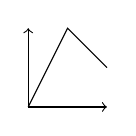
\begin{tikzpicture}\draw[->] (0,0) -- (1,0); \draw[->] (0,0) -- (0,1);\draw (0,0) -- (0.5,1) -- (1,0.5);\end{tikzpicture}$\quad$
            zu viele $b$'s: 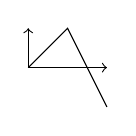
\begin{tikzpicture}\draw[->] (0,0.5) -- (1,0.5); \draw[->] (0,0.5) -- (0,1);\draw (0,0.5) -- (0.5,1) -- (1,0);\end{tikzpicture}
            \begin{flalign*}
            	|w|_a &= |w|_b \rightarrow |f(w)|_a = \frac{3|w|}{2} + \frac{2|w|}{2} = \frac{5}{2}|w|&\\
            	|f(w)|_b &= \frac{|w|}{2} + 2|w| = \frac{5}{2}|w|&\\
            \end{flalign*}
\section{Was macht L schwer?}
    $\rightarrow$ Variable Steigung\\
    Bsp. kann verallgemeinert werden
    \subsection{Definition}
        Zustand q hat \underline{konstante Steigung}, wenn $\exists \alpha \in \mathbb{Q}$ ($\alpha$: Steigung) $\forall w \in \Sigma^*$ mit $$ (q,h_1) \xrightarrow{w} (q,h_2)\text{ und}$$
        $\forall w'$ Präfix von $w: h_1 + \Delta(w') \geq m$ gilt:
        $$h_2 = \alpha|w|+h_1 \text{ Steigung}$$
        \begin{tikzpicture}
        	\tikzstyle{dot}=[draw,circle,fill = black, inner sep=0pt,minimum size=2pt]
        	\draw[->] (0,0) -- (5,0);
        	\draw[->] (0,0) -- (0,5);
        	\draw (0,1) -- (-0.1,1) node [left] {$m$};
        	\draw (0,2) -- (-0.1,2) node [left] {$h_1$};
        	\draw (0,4) -- (-0.1,4) node [left] {$h_2$};
        	\node[dot,right] at (1,2) {};
        	\node[dot,right] at (4,4) {};
        	\draw[dashed] (1,2) -- (4,4) node [midway,below] {$\alpha$};
        	\draw plot[smooth] coordinates {(1,2) (1.8,1.6) (2, 3) (2.5, 4) (3,3.5) (3.7, 3.5) (4,4)};
        	\node[left] at (1,2) {$q$};
        	\node[right] at (4,4) {$q$};
        \end{tikzpicture}\\
        Äquivalent (``Korridor''): $$\exists\alpha\in\mathds{Q},\gamma\in\mathds{N}\forall w\in\Sigmas,w'\text{ Präfix von }w:\alpha|w'|-\gamma\le\Delta(w')\le\alpha|w'|+\gamma$$
